\section{ Понятие правильной нормальной производной. Существование правильной нормальной производной у потенциала простого слоя с непрерывной плотностью. Формула для скачка для нормальной производной.}
Мотивация: во внутренней задаче Неймана (билет 14) ищется решение $u(x) \in C^2(\Omega) \cap C^1(\overline{\Omega})$ уравнения $$\Delta u = f(x), \, x \in \Omega,$$ при условии $$\frac{\partial u}{\partial \vec{n}}\bigg|_{\Gamma} = u_1(x),$$ где $u_1 \in C(\Gamma)$.

Но существуют примеры гармонических в области функций, градиент которых нельзя продолжить по непрерывности на замыкание этой области. Можно расширить понятие классического решения.

    Пусть $u(x) \in C^1(\Omega) \cap C(\overline{\Omega}), \, \Omega$ -- ограниченная область в $\R^3$ с границей $\Gamma \in C^2$.
\begin{center}
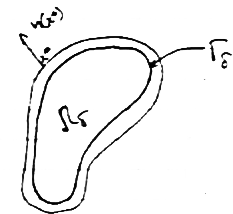
\includegraphics[width=0.2\textwidth]{32_1_new}
\end{center}
Пусть $x^0 \in \Gamma$, а $\vec{n}(x^0)$ -- нормаль к $\Gamma$ в $x^0$. Т.к. $\Gamma \in C^2$, $\vec{n}(x^0)$ -- непрерывная функция по $x^0$. Проведем через $x^0$ прямую $x = x^0 + \vec{n}(x^0)t, \, t \in \mathbb{R}$.

Распишем произведенеие $$(\vec{n}(x^0), \nabla u(x)) = \sum_{k=1}^{3} n_k(x^0)\frac{\partial u}{\partial x_k}(x) = \frac{du(x^0 + \vec{n}(x^0)t)}{dt} = \frac{\partial u}{\partial \vec{n}(x^0)}(x)$$

\begin{definition}
Говорят, что $u(x)$ имеет \textbf{правильную нормальную производную} по направлению внешней нормали на $\Gamma$ из $\Omega$, если  
\begin{enumerate}
\item $\forall x^0 \in \Gamma$ существует конечный предел 
$$\frac{\partial u}{\partial \vec{n}}(x^0) \equiv \lim_{x = x^0 + \vec{n}(x^0)t,\\ x \in \Omega, \\ x \to x^0} \frac{\partial u}{\partial \vec{n}(x^0)}(x)$$

\item Этот предел равномерный по $x^0 \in \Gamma$
\end{enumerate}
\end{definition}
\begin{lemma}
Если u(x) имеет ПНП по нормали $\vec{n}(x^0)$ из $\Omega$ на $\Gamma$, то 
\begin{enumerate}
\item u(x) имеет обычную производную по нормали $\vec{n}(x^0)$ в точке $x^0 \in \Gamma$, и эта производная совпадает с ПНП 

\item ПНП $\in C(\Gamma)$
\end{enumerate}
\end{lemma}
\begin{proof} Обычная производная по нормали $$\lim_{x \to x^0, x = x^0 + \vec{n}(x^0)t} \frac{u(x^0) - u(x)}{|x^0 - x|} = \lim_{t < 0, t \to 0} \frac{u(x^0) - u(x^0 + \vec{n}(x^0)t)}{-t} = \lim_{t < 0, t \to 0} \frac{du(x^0 + \vec{n}(x^0)t)}{dt} = \frac{\partial u}{\partial \vec{n}}(x^0)$$ -- этот предел существует по условию.

Покажем непрерывность: Пусть $\delta$ мало, $0 < \delta < \delta_0, x = x^0 - \delta n(x^0)$

Пусть $V_{\delta}(x^0) = \frac{\partial u}{\partial \vec{n}(x^0)}(x^0 - \delta \vec{n}(x^0))= $

$$=\sum_{k=1}^{3} n_k(x^0)\frac{\partial u}{\partial x_k}(x^0 - \delta \vec{n}(x^0)) \Rightarrow V_{\delta}(x^*) \in C(\Gamma) $$

$n_k(x^0)$ непрерывна, т.к. $\Gamma \in C^2$

По определению ПНП: $V_{\delta} \rightrightarrows $ ПНП $\Rightarrow$ она также непрерывная на $\Gamma$. 
\end{proof}
$\bullet$ После расширения определения классического решения встает вопрос о единственности решения. При исследовании этого вопроса мы использовали формулы Грина. Дли них требовалось гладкость $C^2(\Omega) \cap C^1(\overline{\Omega})$. Покажем, как обобщить эти факты с помощью ПНП.

$\bullet$ Пусть $\Omega$ -- ограниченная область с границей $\R^3$, граница $\Gamma \in C^2, \, 0 < \delta < \delta_{\mu}$

$\Gamma_{\delta} = \{x: x = x^0 - \delta \vec{n}(x^0)\}$ -- граница класса уже $C^1$, т.к. $\vec{n}(x^0) \in C^1$
\begin{center}
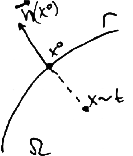
\includegraphics[width=0.2\textwidth]{32_2_new}
\end{center}
\begin{lemma}
Пусть $\Omega$ -- ограниченная область с границей $\Gamma \in C^2, \, u(x) \in C^2(\Omega) \cap C(\overline{\Omega})$, а у $u(x) \Exists $ ПНП по направлению внешней нормали $\vec{n}(x^0), \Delta u \in C(\Omega)$. Тогда $$\int_{\Omega} \Delta u(x) \cdot u(x) \, dx = \oint_{\Gamma} \frac{\partial u}{\partial \vec{n}}(x) \cdot u(x) \, dS - \int_{\Omega} |\nabla u(x)|^2 \, dx $$
\end{lemma}
\begin{proof}
$u(x) \in C^2(\Omega) \cap C(\overline{\Omega}) \Rightarrow u(x) \in C^2(\Omega_{\delta}) \cap C^1(\overline{\Omega_{\delta}}) \Rightarrow $

$$\int_{\Omega_{\delta}} \Delta u(x) \cdot u(x) \, dx (1) = \oint_{\Gamma_{\delta}} \frac{\partial u}{\partial \vec{n}}(x) \cdot u(x) \, dS (2) - \int_{\Omega_{\delta}}|\nabla u(x)|^2 \, dx (3)$$

$\lim_{\delta \to 0}(1) = \int_{\Omega} \Delta u(x)  \cdot u(x) \, dx$, т.к. $\Delta u(x)$ и $u(x) \in C(\overline{\Omega})$

$\lim_{\delta \to 0}(2) = \int_{\Gamma} \frac{\partial u}{\partial \vec{n}}(x) \cdot u(x)dS $

$\lim_{\delta \to 0}(3) = \lim\limits_{x = x^0 - \delta \vec{n}(x^0), \delta \to 0} \int_{\Omega_{\delta}} |\nabla u(x)|^2dx$

$\bullet$ С учетом сделанного обобщения все сделанные ранее рассуждения о внутренних и внешних задачах верны и для расширенного понятия классического решения.
\end{proof}
\begin{theorem}[Корректная постановка внутренней задачи Неймана для уравнения Лапласа]
$\Omega$ -- ограниченная область, граница $\Gamma \in C^2$. Найти функцию $u(x) \in C^2(\Omega) \cap C(\overline{\Omega})$, имеющую ПНП и удовлетворяющую 

\begin{equation}
\begin{cases}
\Delta u(x) = 0, &x \in \Omega,
\\
\frac{\partial u}{\partial \vec{n}}\big|_{\Gamma} = u_1(x) \in C(G).
\end{cases}
\end{equation}
\end{theorem}
\begin{theorem}[Корректная постановка внешней задачи Неймана для уравнения Лапласа]
$\Omega$ -- внешняя область, граница $\Gamma \in C^2$. Найти функцию $u(x) \in C^2(\Omega) \cap C(\overline{\Omega})$ имеющую ПНП и удовлетворяющую 
\begin{equation}
\begin{cases}
\Delta u(x) = 0, &x \in \Omega,
\\
\frac{\partial u}{\partial \vec{n}}\big|_{\Gamma} = u_1(x) \in C(\Gamma),
\\
u(x)|_{x \to \infty} \to 0.
\end{cases}
\end{equation}
\end{theorem}
$\bullet$ Рассмотрим потенциал простого слоя

$\Omega$ -- ограниченная область с границей $\Gamma \in C^2; \, x = x^0 - \delta \vec{n}(x^0); \, 0 < \delta < \delta^*$
  $$V^{(0)} = \int_{\Gamma} \frac{\mu(y)}{|x - y|}dS_y$$

$$\frac{\partial V^{(0)}}{\partial \vec{n}(x^0)}(x) = \sum_{k = 1}^3 n_k(x^0) \frac{\partial}{\partial x_k}\oint_{\Gamma} \frac{\mu(y)}{|x - y|}dS_y = \sum_{k = 1}^3 n_k(x^0) \oint_{\Gamma}  \frac{\partial}{\partial x_k} \left( \frac{1}{|x - y|} \right) \cdot\mu(y)dS_y = $$

$$ = \oint_{\Gamma} \sum_{k = 1}^3 n_k(x^0) \frac{\partial}{\partial x_k} \left( \frac{1}{|x - y|}\right) \cdot \mu(y)dS_y = \oint_{\Gamma} \sum_{k = 1}^3 n_k(x^0) \frac{y_k - x_k}{|x - y|^3}\mu(y)dS_y = \oint_{\Gamma} \frac{(y - x, \vec{n}(x^0))}{|x - y|^3}\mu(y)dS_y$$

Обозначим $\left( \frac{\partial V^{(0)}}{\partial \vec{n}(x^0)} \right)_{\pm}(x^0) = \lim\limits_{x = x^0 \mp \delta \vec{n}(x), \delta \to +0} \frac{\partial V^{(0)}}{\partial \vec{n}(x^0)} (x)$

$\frac{\partial V^{(0)}}{\partial \vec{n}(x^0)}(x^0)(1) = \int_{\Gamma} \frac{(y - x^0, \vec{n}(x^0))}{|x^0 - y|^3}\mu(y)dS_y, x^0 \in \Gamma (2)$

(1) -- прямое значение нормальной производной

(2) -- полярное ядро $\Rightarrow$ $\forall \mu(x) \in C(\Gamma), \Forall x^0 \in \Gamma$ этот интеграл существует, и более того $(1) \in C(\Gamma)$

\begin{theorem}
У потенциала простого слоя $V^{(0)}(x)$ с плотностью $\mu(x) \in C(\Gamma)$ существует ПНП на $\Gamma$: $$\left( \frac{\partial V^{(0)}}{\partial \vec{n}(x^0)}\right)_+(x^0)
\text{ и } \left(\frac{\partial V^{(0)}}{\partial \vec{n}(x^0)}\right)_-(x^0) ,$$
причем имеет место формула скачка 

$$\left(\frac{\partial V^{(0)}}{\partial \vec{n}(x^0)}\right)_{\pm}(x^0) = \frac{\partial V^{(0)}}{\partial \vec{n}(x^0)}(x^0) \pm 2\pi \mu(x^0) $$
\end{theorem}
\begin{conseq}
$\left(\frac{\partial V^{(0)}}{\partial \vec{n}(x^0)} \right)_+(x^0) - \left(\frac{\partial V^{(0)}}{\partial \vec{n}(x^0)} \right)_-(x^0) = 4\pi \mu(x^0), \, x^0 \in \Gamma$

$\frac{\partial V^{(0)}}{\partial \vec{n}(x^0)}(x^0) = \frac{1}{2} \left[ \left(\frac{\partial V^{(0)}}{\partial \vec{n}(x^0)} \right)_+(x^0) + \left(\frac{\partial V^{(0)}}{\partial \vec{n}(x^0)} \right)_-(x^0)\right], \, x \in \Gamma$
\end{conseq}
